%!Mode:: "TeX:UTF-8"
%\begin{frame}
%    \frametitle{OUTLINE}
%    \begin{itemize}    
%        \item
%    \end{itemize}
%\end{frame}

\begin{frame}
    \begin{center}
        \LARGE \tt{GIT}
    \end{center}
\end{frame}

\begin{frame}
    \frametitle{Git基础\footnote{\url{http://git-scm.com/book/en/Getting-Started-Git-Basics}}}
    \begin{itemize}    
        \item 版本控制的概念
        \item 一个重要概念
            \begin{itemize}
                \item Git关心文件数据的整体是否发生变化。
                \item 其他版本管理系统则关心具体内容的差异。
            \end{itemize}
    \end{itemize}
\end{frame}

\begin{frame}
    \frametitle{git的版本控制模型}
    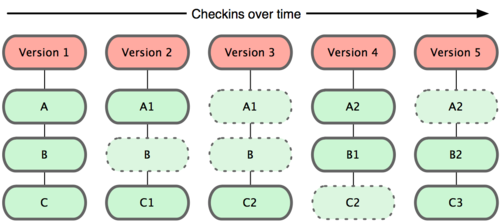
\includegraphics[width=10cm,keepaspectratio]{data/GitRevisionModel.png}
\end{frame}

\begin{frame}
    \frametitle{其他系统的版本控制模型}
    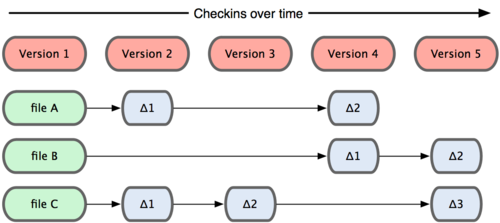
\includegraphics[width=10cm,keepaspectratio]{data/OtherRevisionModel.png}
\end{frame}

\begin{frame}
    \frametitle{Git项目仓库}
    \begin{itemize}    
        \item 创建一个仓库
            \begin{itemize}
                \item 在工作目录中初始化新仓库
                \item 从现有仓库克隆
            \end{itemize}
        \item 在 Git 中的绝大多数操作都只需要访问本地文件和资源。
        \item 我们每个人的工作目录,都有整个仓库的完整信息。
    \end{itemize}
\end{frame}

\begin{frame}
    \frametitle{分布式工作流程\footnote{\url{http://git-scm.com/book/en/Distributed-Git-Distributed-Workflows}}}
    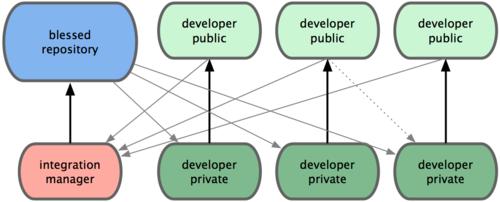
\includegraphics[width=10cm,keepaspectratio]{data/GitDistributedWorkflow.png}
\end{frame}

\begin{frame}
    \frametitle{Git的数据流}
    \begin{columns}
        \column{6.0cm}
            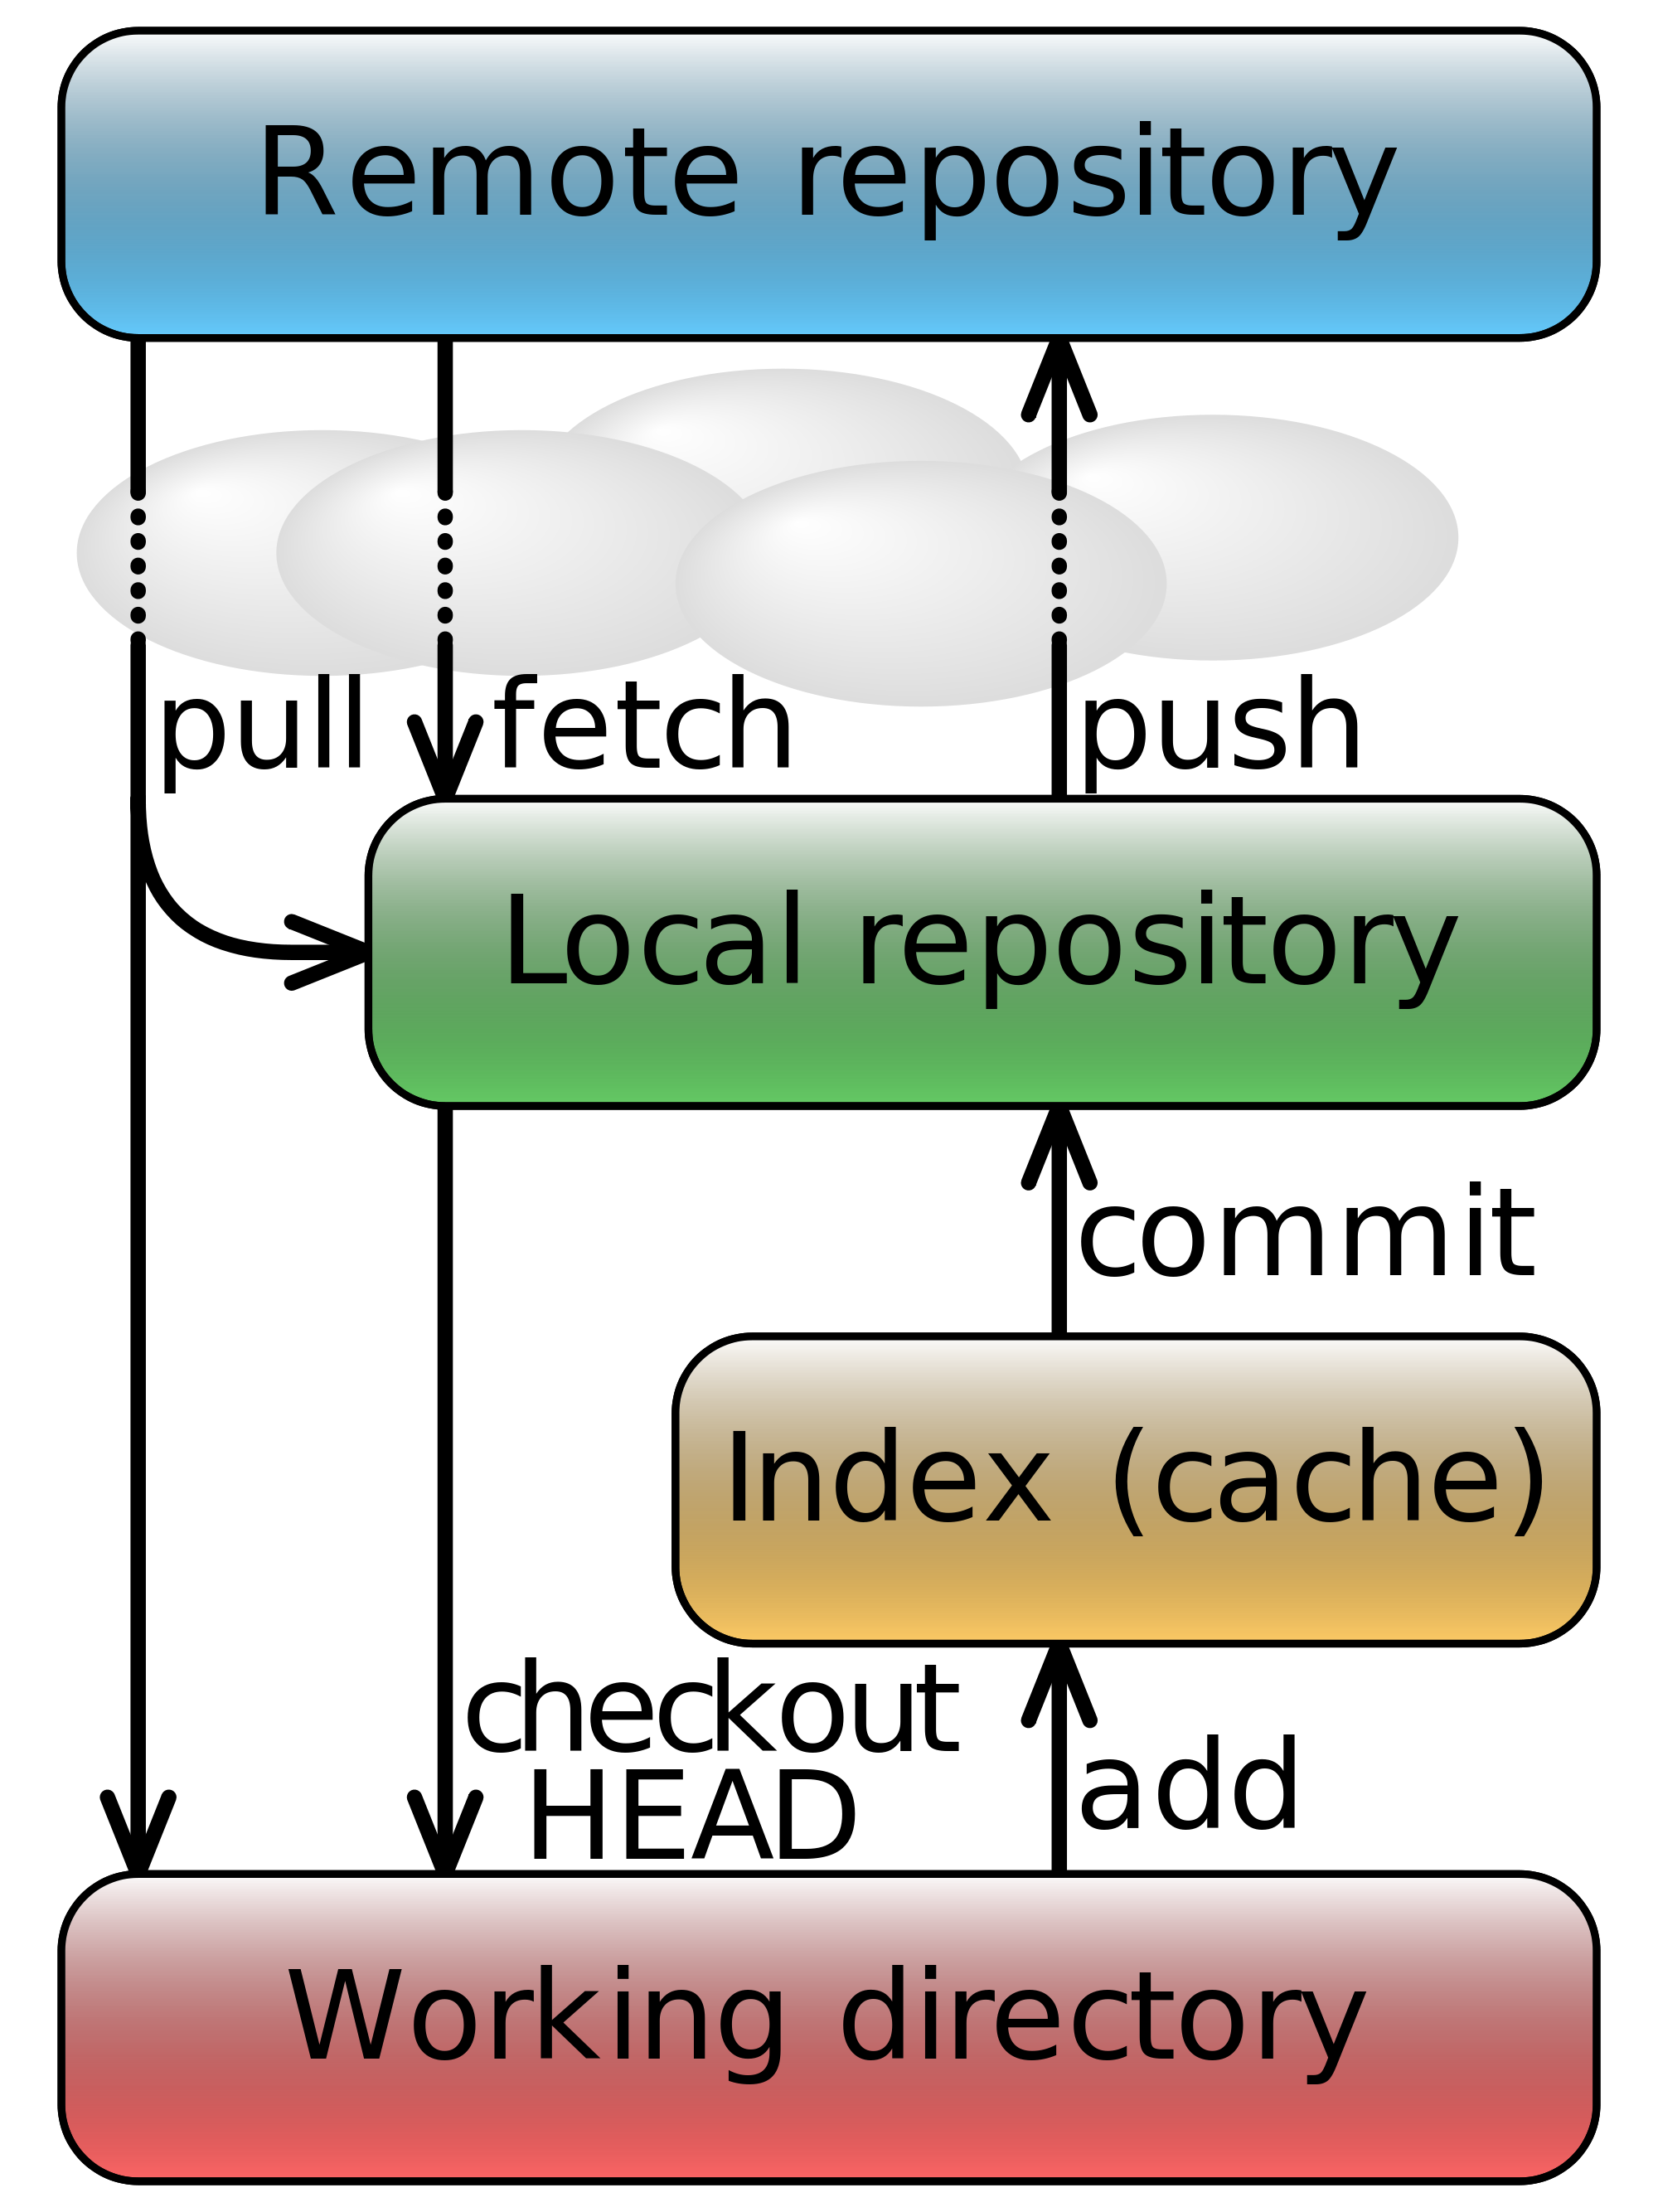
\includegraphics[height=8cm,keepaspectratio]{data/GitDataFlowSimplified.png}
            \label{pic:DataFlow}
        \column{4.5cm}
            \begin{itemize}
                \item 远程仓库
                \item 本地仓库
                \item 工作目录
            \end{itemize}
    \end{columns}
\end{frame}

\begin{frame}
    \frametitle{Git的基本命令}
    \begin{itemize}    
        \item 了解了第\ref{pic:DataFlow}页的图形后,命令就简单了。
        \item \tt{git clone}
        \item \tt{git commit}
        \item \tt{git pull}
        \item \tt{git push}
    \end{itemize}
\end{frame}

\begin{frame}
    \frametitle{示例}
    \begin{itemize}    
        \item \tt{\footnotesize{git clone git@host:users/lintao/Dyb2Sim.git}}
        \item \tt{\footnotesize{git commit -am "Add an comment."}}
        \item 多commit!记录每个细节!
        \item \tt{\footnotesize{git pull origin}}
        \item \tt{\footnotesize{git push origin master}}
    \end{itemize}
\end{frame}

\begin{frame}
    \frametitle{关于origin}
    \begin{itemize}
        \item \tt{origin}表示远程仓库的名字
        \item \tt{\footnotesize{git remote}}看有哪些仓库
        \item \tt{\footnotesize{git remote show origin}}看仓库的具体信息
        \item 我们可以加入\emph{多个}远程仓库
    \end{itemize}
\end{frame}

\begin{frame}
    \frametitle{关于master}
    \begin{itemize}
        \item \tt{master}表示\emph{分支}的名字
        \item 分支是什么?
        \item 简单来说,分支就是我们\tt{commit}时的历史。
        \item 创建新分支
            \begin{itemize}
                \item \tt{\footnotesize{git checkout -b testing}}
            \end{itemize}
        \item 切换分支
            \begin{itemize}
                \item \tt{\footnotesize{git checkout master}}
            \end{itemize}
    \end{itemize}
\end{frame}

\begin{frame}
    \frametitle{来自\tt{git-scm.com}\footnote{\url{http://git-scm.com/book/en/Git-Branching-What-a-Branch-Is}}}
    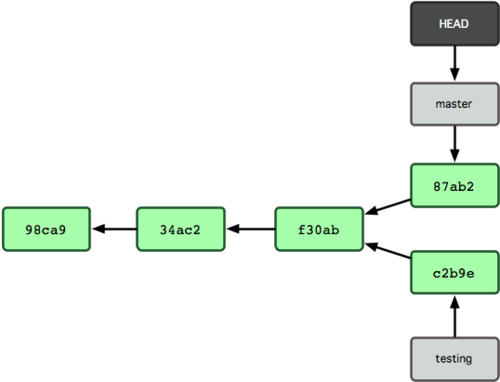
\includegraphics[height=6cm,keepaspectratio]{data/GitBranch.png}
\end{frame}

\begin{frame}
    \frametitle{更多关于分支}
    \begin{itemize}    
        \item Git的分支是轻量级的
        \item 实验某个功能,{\LARGE多用}分支
        \item 可以很简单的进行{\LARGE合并}
            \begin{itemize}
                \item \tt{\footnotesize{git merge testing}}
            \end{itemize}
    \end{itemize}
\end{frame}


\newsavebox{\TryGitBranch}
\begin{lrbox}{\TryGitBranch}
\begin{lstlisting}
$ mkdir TestBranch; cd TestBranch
$ git init
$ touch README
$ git add README
$ git commit -am "Add README"
$ (*@\hl{git checkout -b testing}@*)
$ touch README-IN-TESTING
$ git add README-IN-TESTING
$ git commit -am "in testing"
$ (*@\hl{ls}@*)
$ git checkout master
$ (*@\hl{ls}@*)
\end{lstlisting}
\end{lrbox}

\begin{frame}
    \frametitle{亲自试试}
    \par\usebox{\TryGitBranch}
\end{frame}

\begin{frame}
    \frametitle{哪里神奇了?}
        \begin{itemize}
            \item 如果大家比较两个\tt{ls}的结果,会发现什么?
            \item 在分支testing中修改的东西,并不影响master。
            \item 所以,大家可以放心的创建和使用分支功能。
        \end{itemize}
\end{frame}

\begin{frame}
    \frametitle{Git小结}
        \begin{itemize}
            \item 多去使用,自然就习惯了
            \item 多\tt{git commit},让git去记录你工作的细节
            \item 多\tt{git checkout},别再为了一个新概念的工作
                  而重新拷贝代码了,交给git吧
        \end{itemize}
\end{frame}
